\section{Datastruktur}
\label{sec:datastruktur}
I implementeringen af ethvert kort må den bagvedliggende datastruktur nøje overvejes, da denne i høj grad afgør applikationens ressourcekrav. Overvejelserne omkring datastrukturen involverede blandt andet muligheden for kun at indlæse specifikke dele af dataet samt søgeegenskaber. Det givne datasæt består af knudepunkter og tilhørende vejsegmenter, som forbinder to af disse knudepunkter. Knudepunkterne indeholder information om deres individuelle placering, mens vejsegmenterne er forbundet med en række forskellige oplysninger såsom vejnavn og -type. Da kortdataet består af vejsegmenter, er det også af betydning for valget af datastruktur. Værd at overveje var også datastørrelsen --- datakilden fra Krak indeholder over en million knudepunkter, og disse skal på ethvert tidspunkt under programkørslen kunne tilgås, hurtigt.

Flere forskellige datastrukturer syntes besidde de nævnte egenskaber: heriblandt en sorteret tabel, et k-d træ og en quadtree-struktur. Den sorterede tabel brillerer med en ukompliceret implementering. Quadtree og k-d træ, mens komplicerede at implementere, udmærker sig derimod ved deres simple datasegmentering samt hastige indlæsning af specifikke områder.

K-d træet splittes ved median elementet og opdeler træet i to subproblemer. Der splittes igen omkring median elementet i hvert subproblem, hvortil der opstår to subproblemer per split. I en quadtree-struktur, derimod, indeholder hver \emph{quad} fire andre quads --- NØ, SØ, SV og NV. Individuelle quads kan acceptere et begrænset antal elementer, hvorefter ethvert fremtidigt forsøg på indsættelse vil blive videregivet til dennes indholdte quads rekursivt.
\begin{figure}[ht]
	\centering
	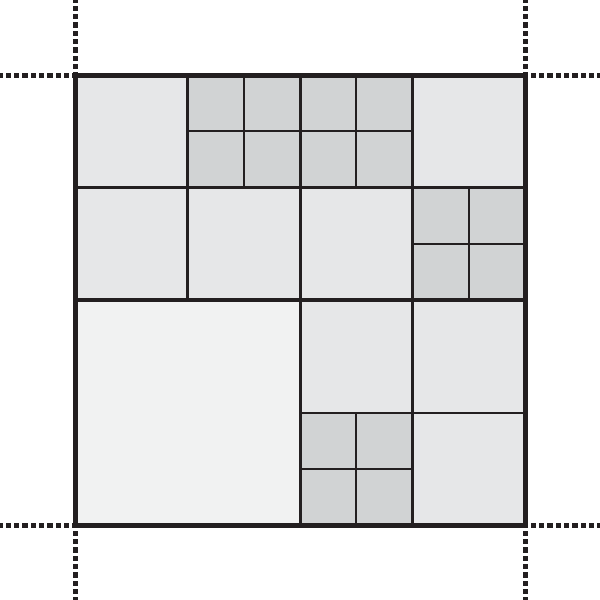
\includegraphics[width=0.5\textwidth]{quadtree1}
	\captionsetup{width=0.8\textwidth}
	\caption{Eksempel på udsnit en quadtree-struktur hvori dybden af de individuelle quads fremhæves af disses nuance.}
	\label{fig:quadtree1}
\end{figure}
Elementforespørgsel, hvor et rektangulært område søges, foregår ligeledes rekursivt. En quad, som modtager en forespørgsel, vil forespørge sine indholdte quads om selvsamme, og derefter returnere resultatet af dette sammenlagt med sine egne elementer.

Det vurderes at en sorteret liste ville være for langsom til vores behov. Det var svært at sætte fingeren på en konkret forskel i ydeevnen mellem k-d træet og quadtree-strukturen. Grundet et langt større kendskab til quadtree-strukturens virkemåde, sås denne således som den mest passende løsning. Vi fandt det vigtigt at valget og udarbejde datastrukturen hurtigt, da udviklingen af resten af programmet afhang deraf.

\subsection{Linjeplacering}
\begin{figure}[ht]
	\centering
	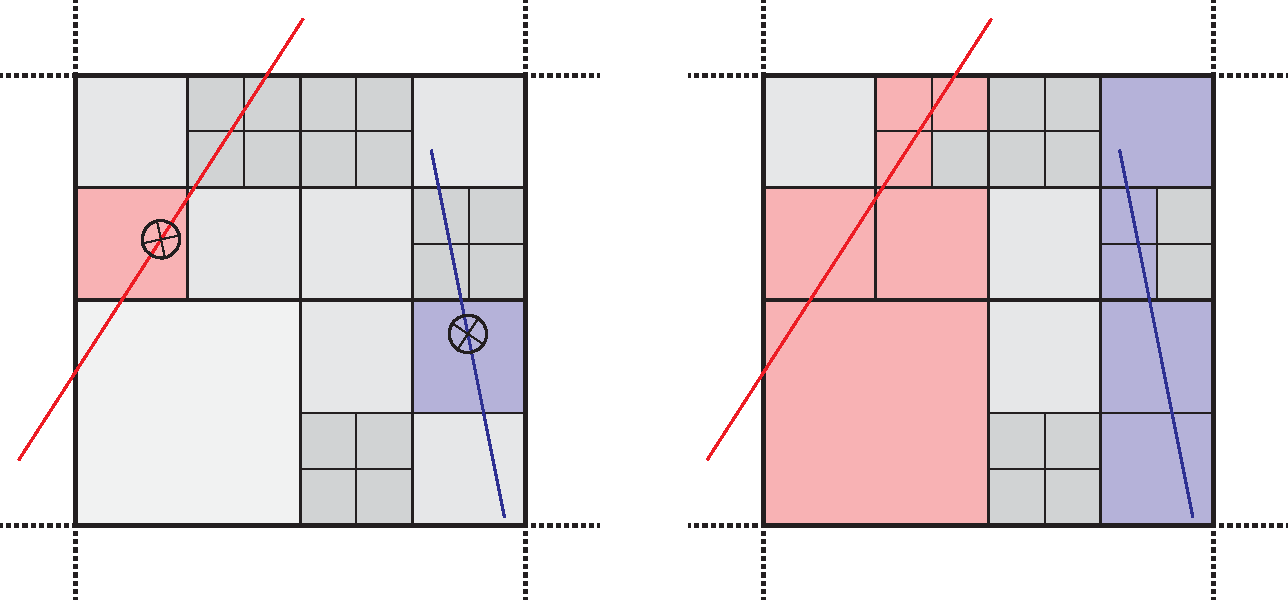
\includegraphics[width=0.5\textwidth]{quadtree2}
	\captionsetup{width=0.8\textwidth}
	\caption{CAPTION}
	\label{fig:quadtree2}
\end{figure}
\begin{figure}[ht]
	\centering
	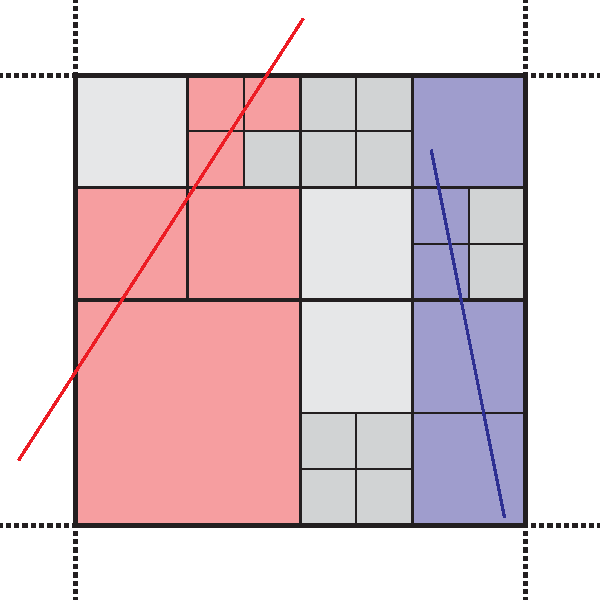
\includegraphics[width=0.5\textwidth]{quadtree3}
	\captionsetup{width=0.8\textwidth}
	\caption{CAPTION}
	\label{fig:quadtree3}
\end{figure}